%----------------------------------------------------------------------------------
% Exemplo do uso da classe tcc.cls. Veja o arquivo .cls
% para mais detalhes e instruções.
%----------------------------------------------------------------------------------

% Seleção de idioma da monografia. Por enquanto as únicas opções
% suportadas são 'portuguese' e 'english'
% Para impressão em frente e verso, use a opção 'twoside'. Da
% mesma forma, use 'oneside' para impressão em um lado apenas.
\documentclass[portuguese,oneside]{tcc}

%----------------------------------------------------------------
% Coloque seus pacotes abaixo.
%
% Obs.: muitos pacotes de uso comum do LaTeX, como amsmath,
% geometry e url já são automaticamente incluídos pela classe
% (veja o arquivo .cls). Isso torna obrigatória a presença destes
% no sistema para o uso desta classe, mas ao mesmo tempo o uso se
% torna mais simples.  Recomendo a instalação da versão mais
% recente da distribuição TeXLive (para Windows e UNIXes):
% www.tug.org/texlive/
%
% Pacotes e opções já incluídas automaticamente:
%
% \RequirePackage[T1]{fontenc}[2005/09/27]
% \RequirePackage[utf8x]{inputenc}[2008/03/30]
% \RequirePackage[english,brazil]{babel}[2008/07/06]
% \RequirePackage[a4paper]{geometry}[2010/09/12]
% \RequirePackage{textcomp}[2005/09/27]
% \RequirePackage{lmodern}[2009/10/30]
% \RequirePackage{indentfirst}[1995/11/23]
% \RequirePackage{setspace}[2000/12/01]
% \RequirePackage{textcase}[2004/10/07]
% \RequirePackage{float}[2001/11/08]
% \RequirePackage{amsmath}[2000/07/18]
% \RequirePackage{amssymb}[2009/06/22]
% \RequirePackage{amsfonts}[2009/06/22]
% \RequirePackage{url}
% \RequirePackage[table]{xcolor}[2007/01/21]
%----------------------------------------------------------------
% Para inserção de figuras.
\usepackage{graphicx}
% Utilize a opção 'pdftex' se você estiver usando o pdflatex (que
% permite figuras em formatos como .jpg ou .png)
%\usepackage[pdftex]{graphicx}

% Para tabelas com elementos ocupando mais de uma linha
\usepackage{multirow}
% Para frações na mesma linha (ex. ⅓).
\usepackage{nicefrac}
% Para inserir figuras lado a lado.
% \usepackage{subfigure}
% Para formatar algoritmos.
% A opção [algo2e] é necessária para evitar conflitos
% com as definições da classe.
%\usepackage[algo2e]{algorithm2e}
\usepackage{algorithmic}
% Um float do tipo algoritmo. No momento
% este pacote é incompatível com a classe.
%\usepackage{algorithm}

%----------------------------------------------------------------
% Autor (OBRIGATÓRIO)
%----------------------------------------------------------------
\author{Fulano da Silva}

%----------------------------------------------------------------
% Título (OBRIGATÓRIO). Devem ser passados DOIS parâmetros,
% o título em português E o inglês, não importando o idioma
% escolhido. Os títulos são utilizados para a montagem da capa,
% resumo e abstract mais tarde.
%----------------------------------------------------------------
\title{Seu título em português aqui}
      {Your title in english here}

%----------------------------------------------------------------
% Opções para o tipo de trabalho (OBRIGATÓRIO)
%----------------------------------------------------------------
%\tipotrabalho{\ptci}         % Proposta de Trabalho de Conclusão
%\tipotrabalho{\tci}         % Trabalho de Conclusão I
\tipotrabalho{\tcii}        % Trabalho de Conclusão II

%----------------------------------------------------------------
% Seleção do curso ("este trabalho é um requisito parcial para
% obtenção do grau de (mestre ou doutor) em Ciência da Computação").
%----------------------------------------------------------------
\curso{\cc} % Ciência da Computação
%\curso{\si} % Sistemas de Informação
%\curso{\es} % Engenharia de Software

%----------------------------------------------------------------
% Orientador (e Co-orientador, caso haja um). É OBRIGATÓRIO
% informar pelo menos o orientador.
%----------------------------------------------------------------
\orientador{Beltrano Dias}
\coorientador{Ciclano de Farias}

%----------------------------------------------------------------
% A capa é inserida automaticamente. Por isso não é necessário
% chamar \maketitle
%----------------------------------------------------------------
\begin{document}

%----------------------------------------------------------------
% Depois da capa vem a dedicatória e a epígrafe.
%----------------------------------------------------------------
\dedicatoria{Dedico este trabalho a meus pais.}

\epigrafe{The art of simplicity is a puzzle of complexity.}
         {Douglas Horton}

%----------------------------------------------------------------
% Também dá para fazer as duas na mesma página:
%----------------------------------------------------------------
%\dedigrafe{Dedico este trabalho a meus pais.}
%          {The art of simplicity is a puzzle of complexity.}
%          {Douglas Horton}

%----------------------------------------------------------------
% A seguir, a página de agradecimentos (OPCIONAL):
%----------------------------------------------------------------
\begin{agradecimentos}
À lorem ipsum, dolor sit amet consetetur sadipscing elitr sed diam
nonumy eirmod tempor. invidunt ut labore et dolore magna aliquyam

À erad sed, diam voluptua at vero, eos et accusam et justo duo
dolores et ea rebum stet clita.

À kasd gubergren, no sea. takimata sanctus est lorem ipsum dolor sit
amet lorem ipsum dolor sit amet. consetetur sadipscing elitr sed

À diam nonumy, eirmod tempor, invidunt ut labore et dolore magna
aliquyam erat sed diam voluptua at.
\end{agradecimentos}

%----------------------------------------------------------------
% Resumo, com as palavras-chave passadas por parâmetro
% (OBRIGATÓRIO, ao menos para teses e dissertações)
%----------------------------------------------------------------
\begin{resumo}{lorem, ipsum, dolor, sit, amet}
Seu resumo em português aqui. lorem ipsum dolor sit amet
consetetur sadipscing elitr sed diam nonumy eirmod tempor invidunt
ut labore et dolore magna aliquyam erat sed diam voluptua at vero
eos et accusam et justo duo dolores et ea rebum stet clita.  kasd
gubergren no sea takimata sanctus est lorem ipsum dolor sit amet
lorem ipsum dolor sit amet consetetur sadipscing elitr sed diam
nonumy eirmod tempor invidunt ut labore et dolore magna aliquyam
erat sed diam voluptua at.
\end{resumo}

%----------------------------------------------------------------
% Abstract, com as palavras-chave passadas por parâmetro
% (OBRIGATÓRIO, ao menos para teses e dissertações)
%----------------------------------------------------------------
\begin{abstract}{lorem, ipsum, dolor, sit, amet}
Your abstract in English here. lorem ipsum dolor sit amet
consetetur sadipscing elitr sed diam nonumy eirmod tempor invidunt
ut labore et dolore magna aliquyam erat sed diam voluptua at vero
eos et accusam et justo duo dolores et ea rebum stet clita kasd
gubergren no sea takimata sanctus est lorem ipsum dolor sit amet
lorem ipsum dolor sit amet consetetur sadipscing elitr sed diam
nonumy eirmod tempor invidunt ut labore et dolore magna aliquyam
erat sed diam voluptua at
\end{abstract}

%----------------------------------------------------------------
% Listas e sumário, nessa ordem. Somente o sumário é obrigatório,
% portanto, comente as outras listas, caso sejam desnecessárias.
%----------------------------------------------------------------
\listoffigures       % Lista de figuras      (OPCIONAL)
\listoftables        % Lista de tabelas      (OPCIONAL)
\listofalgorithms    % Lista de algoritmos   (OPCIONAL)
\listofacronyms      % Lista de siglas       (OPCIONAL)
\listofabbreviations % Lista de abreviaturas (OPCIONAL)
\listofsymbols       % Lista de símbolos     (OPCIONAL)
\tableofcontents     % Sumário               (OBRIGATÓRIO)

%----------------------------------------------------------------
% Aqui começa o desenvolvimento do trabalho. Para uma melhor
% organização do documento, separe-o em arquivos,
% um para cada capítulo. Para isso, utilize o comando \include,
% como mostrado abaixo.
%----------------------------------------------------------------
%----------------------------------------------------------------------------------
% Exemplo do uso da classe tcc.cls. Veja o arquivo .cls
% para mais detalhes e instruções.
%----------------------------------------------------------------------------------
\chapter{\label{chap:intro}Introdução}
% Comando para inserir siglas. Tanto as siglas quanto as
% abreviaturas devem aparecer em ordem ALFABÉTICA nas listas
% correspondentes. Como a classe no momento não é capaz de ordenar
% as entradas automaticamente, existem duas alternativas:
%
%    a- Insira todas as siglas e abreviaturas no começo do texto,
%    manualmente e em ordem alfabética.
%
%    b- Caso esteja em um ambiente UNIX (Linux, Mac ou Cygwin/similares),
%    utilize o script sort.sh e o makefile que acompanham a
%    classe. O makefile automaticamente compila a monografia para
%    PDF (mas assume que o latex está acessível pela linha de
%    comando). Neste caso a ordenação é feita de forma automática.
%
\sigla{abc}{Associação Brasileira de Computadores}
\sigla{xyz}{lorem ipsum dolor sit}
\sigla{ijk}{lorem ipsum dolor sit}
%
% Comando para inserir abreviaturas.
%
\abrev{Abrev}{Abreviatura}
\abrev{Inform}{Informática}
%
% Comando para inserir símbolos. Estes irão aparecer em ordem
% de ocorrência, já que o número da página está presente na lista
% de símbolos.
\simbolo{Hz}{Hertz}
\simbolo{$\pi$}{Constante com valor aproximado de $3.1415926$}%
%
lorem ipsum dolor sit amet Capítulo~\ref{chap:intro} consetetur
sadipscing elitr sed diam nonumy eirmod tempor invidunt ut labore
et dolore magna aliquyam erat sed diam voluptua at vero eos et
accusam et justo duo dolores et ea rebum stet clita kasd gubergren
no sea takimata sanctus est lorem ipsum dolor sit amet lorem ipsum
dolor sit amet consetetur sadipscing elitr sed diam nonumy eirmod.
Ver Figura~\ref{fig:fig1}.

% Um exemplo de figura
\begin{figure}[htb!]
\centering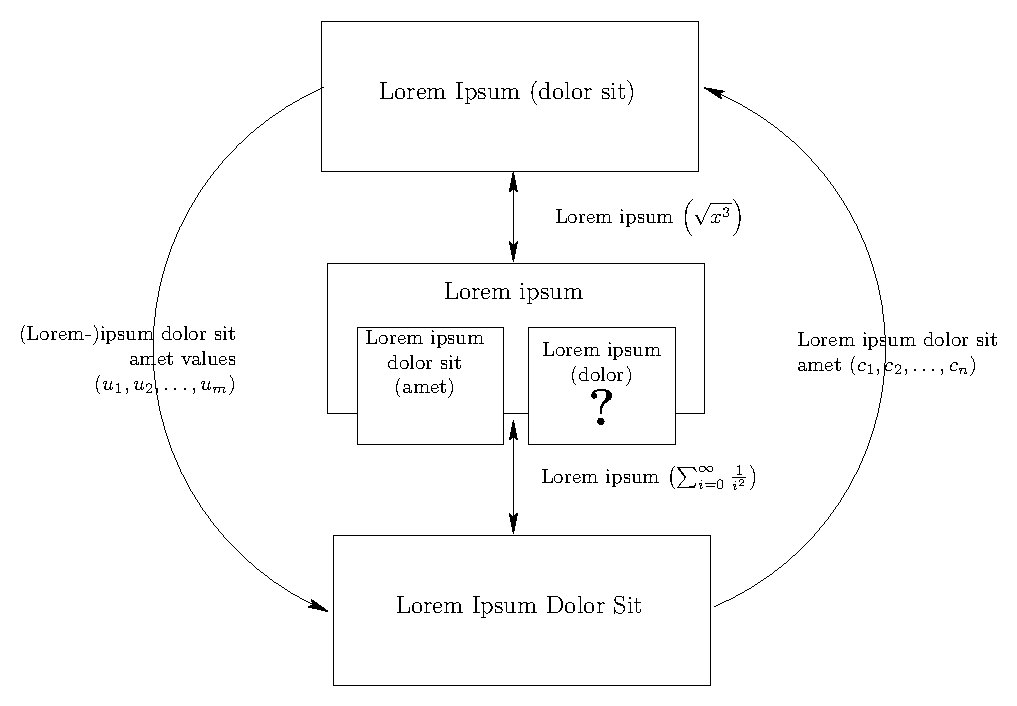
\includegraphics[width=.65\textwidth]{fig/exemplo.eps}
\caption%[This figure has a shorter caption now]%
        {\label{fig:fig1}This is a figure with a very long
    caption which looks ugly in the corresponding list of figures.
    Fortunately, there is an optional parameter for a shorter
    replacement of this monstrosity}%
\end{figure}

tempor invidunt~\cite{SKIENAC698} ut labore et dolore magna
aliquyam erat sed diam voluptua at vero eos et accusam et justo
duo dolores et ea rebum stet clita kasd gubergren no sea takimata
sanctus est lorem ipsum dolor sit amet lorem
ipsum~\cite{NAGAPACKING07}. O Algoritmo~\ref{alg:alg1}
mostra este processo.

\begin{algorithm}[htb]
\begin{center}
    % Um exemplo de algoritmo utilizando a pacote 'algorithmic'
    %\algsetup{linenosize=\small,linenodelimiter=.}
    \begin{algorithmic}[1]
        \STATE \textbf{function} $\sigma\left(i,j\right)$
        \STATE \COMMENT{\texttt{table} lorem ipsum dolor consetetur sadipscing elitr sed $\left(i,j\right)$}
        \IF{$\text{table}\left[i,j\right].\text{memoized}$}
            \RETURN $\text{table}\left[i,j\right].\text{error}$
        \ENDIF
        \STATE $\text{minerror}\leftarrow\infty$
        \STATE $\text{bestt}\leftarrow{}\text{nil}$
        \FOR { each template $t$ in $T$ }
            \STATE $\text{error}\leftarrow{}\text{allocate}\left(t,i,j\right)$
            \IF{$\text{error}<\text{minerror}$}
                \STATE $\text{minerror}\leftarrow{}\text{error}$
                \STATE $\text{bestt}\leftarrow{}t$
            \ENDIF
        \ENDFOR
        \STATE $\text{table}\left[i,j\right].\text{memoized}\leftarrow{}\text{true}$
        \STATE $\text{table}\left[i,j\right].\text{template}\leftarrow{}\text{bestt}$
        \STATE $\text{table}\left[i,j\right].\text{error}\leftarrow{}\text{minerror}$
        \RETURN $\text{minerror}$
    \end{algorithmic}
\end{center}
\caption[An algorithm with an optional, shorter caption]%
    {\label{alg:alg1}This is an algorithm with a very long
    caption. However, we replaced it with a shorter version
    in the Outline for legibility reasons}%
\end{algorithm}

tempor invidunt ut labore et dolore magna aliquyam erat sed diam
voluptua at vero eos et accusam et justo duo dolores et ea
rebum~\cite{CORMEMALGORITHMS01}.

dolor sit~\cite{BENTLEYBC07} amet consetetur sadipscing elitr sed
diam nonumy eirmod tempor invidunt ut labore et dolore magna
aliquyam erat sed diam voluptua at vero~\cite{BRIANPL04}.

\begin{enumerate}
   \item lorem
   \item ipsum
   \item dolor
   \item sit
   \item amet
   \item consetetur
\end{enumerate}

\section{\label{sec:secao1}Primeira seção}

lorem ipsum dolor sit $x\leq 2$  amet consetetur sadipscing elitr
sed diam nonumy eirmod Seção~\ref{sec:secao1} tempor invidunt ut
labore et dolore magna aliquyam erat sed diam voluptua at vero eos
et accusam et justo duo dolores et ea rebum stet
clita.~\cite{OLIVEIRAAPL08}

% Um exemplo de fórmula
\begin{equation}\label{eq:eq1}
    \intop_{0}^{\infty}{x^2 + \frac{\pi}{\sum_{i=0}^{n}{\frac{1}{i^2}}}}
\end{equation}

kasd gubergren no sea Equação~\eqref{eq:eq1} takimata sanctus est
lorem ipsum dolor sit amet lorem ipsum dolor sit amet consetetur
sadipscing elitr sed diam nonumy eirmod.~\cite{PICCOLIAPL11}

amet lorem ipsum dolor sit amet consetetur sadipscing elitr sed
diam nonumy eirmod.~\cite{PICCOLIDM08}

\subsection{Subseção}

dolor sit amet consetetur sadipscing elitr sed diam nonumy eirmod
tempor invidunt ut labore et dolore magna aliquyam erat sed diam
voluptua at vero.

lorem ipsum dolor sit amet consetetur sadipscing elitr sed diam
nonumy eirmod tempor invidunt ut labore et dolore magna aliquyam
erat sed diam voluptua at vero eos et accusam et justo duo dolores
et ea rebum stet clita kasd gubergren no sea takimata sanctus est
lorem ipsum dolor sit amet lorem ipsum dolor sit amet consetetur
sadipscing elitr sed diam nonumy eirmod.

tempor invidunt ut labore et dolore magna aliquyam erat sed diam voluptua at
vero eos et accusam et justo duo dolores et ea rebum stet clita kasd
gubergren no sea takimata sanctus est lorem ipsum dolor sit amet lorem ipsum
dolor sit amet consetetur sadipscing elitr sed diam nonumy eirmod tempor
invidunt ut labore et dolore magna aliquyam erat sed diam voluptua
at vero:

\begin{itemize}
   \item lorem
   \item ipsum
   \item dolor
   \item sit
   \item amet
   \item consetetur
\end{itemize}

\subsubsection{Subsubsub}

lorem ipsum dolor sit amet consetetur sadipscing elitr sed diam nonumy
eirmod tempor invidunt ut labore et dolore magna aliquyam erat sed diam
voluptua at vero eos et accusam et justo duo dolores et ea rebum
stet clita.~\cite{GOLDENBERGAPL02}

\begin{equation}\label{eq:apl}%
    L\left(i,j,w,h\right)=
    \begin{cases}
      E\left(i,w,h\right) & i=j\\
      \min\left(\min_{k=i}^{j-1}\left\{\heartsuit\left(i,k,j,w,h\right)\right\},
                \min_{k=i}^{j-1}\left\{\spadesuit\left(i,k,j,w,h\right)\right\}\right) & i<j\text{.}
    \end{cases}
\end{equation}

lorem ipsum dolor sit amet consetetur sadipscing elitr sed diam nonumy
eirmod tempor invidunt ut labore et dolore magna aliquyam erat sed diam
voluptua at vero eos et accusam et justo duo dolores et ea rebum stet clita
kasd gubergren no sea takimata sanctus est lorem ipsum dolor sit amet lorem
ipsum dolor sit amet consetetur sadipscing elitr sed diam nonumy eirmod
tempor invidunt ut labore et dolore magna aliquyam erat sed diam voluptua at
vero eos et accusam et justo duo dolores et ea rebum stet clita kasd
gubergren no sea takimata sanctus est lorem ipsum dolor sit amet lorem ipsum
dolor sit amet consetetur sadipscing elitr sed diam nonumy eirmod tempor
invidunt ut labore et dolore magna aliquyam erat sed diam voluptua at vero
eos et accusam et justo duo dolores et ea rebum stet clita kasd gubergren no
sea takimata sanctus est lorem ipsum dolor sit amet.

%----------------------------------------------------------------------------------
% Exemplo do ambiente para citações diretas com mais de 3 linhas.
%
% Para citações diretas de até 3 linhas, faça assim:
% De acordo com Direto~(2011, p.~21): "bla bla bla, bla 'bla'."
De acordo com Esquedo~(2011, p.~19):

\begin{directcite}
ut wisi enim ad minim veniam quis nostrud exerci tation ullamcorper suscipit
lobortis nisl ut aliquip ex ea commodo consequat duis autem vel eum iriure
dolor in hendrerit in vulputate velit esse molestie consequat vel illum
dolore eu feugiat nulla facilisis at vero eros et accumsan et
iusto odio
\end{directcite}

duis autem vel eum iriure dolor in hendrerit in vulputate velit esse
molestie consequat vel illum dolore eu feugiat nulla facilisis at vero eros
et accumsan et iusto odio dignissim qui blandit praesent luptatum zzril
delenit augue duis dolore te feugait nulla facilisi lorem ipsum dolor sit
amet consectetuer adipiscing elit sed diam nonummy nibh euismod tincidunt ut
laoreet dolore magna aliquam erat volutpat.

ut wisi enim ad minim veniam quis nostrud exerci tation ullamcorper suscipit
lobortis nisl ut aliquip ex ea commodo consequat duis autem vel eum iriure
dolor in hendrerit in vulputate velit esse molestie consequat vel illum
dolore eu feugiat nulla facilisis at vero eros et accumsan et iusto odio
dignissim qui blandit praesent luptatum zzril delenit augue duis dolore te
feugait nulla facilisi.

nam liber tempor cum soluta nobis eleifend option congue nihil imperdiet
doming id quod mazim placerat facer possim assum lorem ipsum dolor sit amet
consectetuer adipiscing elit sed diam nonummy nibh euismod tincidunt ut
laoreet dolore magna aliquam erat volutpat ut wisi enim ad minim veniam quis
nostrud exerci tation ullamcorper suscipit lobortis nisl ut aliquip ex ea
commodo consequat.

%----------------------------------------------------------------------------------
% Exemplo do uso da classe tcc.cls. Veja o arquivo .cls
% para mais detalhes e instruções.
%----------------------------------------------------------------------------------
\chapter{\label{chap:chap2}Another chapter}

lorem ipsum dolor sit amet consetetur sadipscing elitr sed diam
nonumy eirmod tempor invidunt~\cite{PLASSPAG81} ut labore et
dolore magna aliquyam erat sed diam voluptua at vero eos et
accusam et justo duo dolores et ea rebum stet clita kasd gubergren
no sea takimata sanctus est lorem ipsum dolor sit amet lorem ipsum
dolor sit amet consetetur sadipscing elitr sed diam nonumy eirmod
tempor invidunt ut labore et dolore magna aliquyam erat sed diam
voluptua at vero eos et accusam et justo duo dolores et ea rebum
stet clita kasd gubergren no sea takimata sanctus est lorem ipsum
dolor sit amet lorem ipsum. A Tabela~\ref{tab:tab1} mostra o
cronograma.~\cite{WIKIPIC09}

% Um exemplo relativamente complicado de tabela.
\begin{table}[htb]
\begin{center}
\caption{\label{tab:tab1}This is a table}%
%\rowcolors{4}{black!10}{black!15}
\setlength{\tabcolsep}{.5cm}%
\resizebox{.7\linewidth}{!}{%
\begin{tabular}{r*{2}{>{\columncolor[gray]{0.95}}c>{\columncolor[gray]{1.0}}c}}%
\noalign{\smallskip}
%\hline
\multirow{2}{*}{\textbf{Atividade}} & \multicolumn{4}{c}{\textbf{Ano/Semestre}}\tabularnewline
\cline{2-5}
   & \textbf{2011/II} & \textbf{2012/I} & \textbf{2012/II} & \textbf{2013/I}\tabularnewline
1  &            &            &            &          \tabularnewline
2  & \checkmark & \checkmark & \checkmark &          \tabularnewline
3  & \checkmark & \checkmark & \checkmark &          \tabularnewline
4  & \checkmark & \checkmark & \checkmark & $\times$ \tabularnewline
5  &            &            &            &          \tabularnewline
6  &            &            &            &          \tabularnewline
7  & $\times$   &            &            &          \tabularnewline
8  &            & $\times$   &            &          \tabularnewline
9  &            & $\times$   & $\times$   &          \tabularnewline
10 & $\times$   & $\times$   & $\times$   &          \tabularnewline
11 & $\times$   & $\times$   & $\times$   & $\times$ \tabularnewline
\end{tabular}}
\end{center}
\end{table}

\section{Another section}

Lorem ipsum dolor sit amet consetetur sadipscing elitr sed diam
nonumy eirmod tempor invidunt ut labore et dolore magna aliquyam
erat sed diam voluptua at vero eos et accusam et justo duo dolores
et ea rebum stet clita kasd gubergren no sea takimata sanctus est
lorem ipsum dolor sit amet lorem.~\cite{XIAOAPL05}

Lorem ipsum dolor sit amet consetetur sadipscing elitr sed diam
nonumy eirmod tempor invidunt ut labore et dolore magna aliquyam
erat sed diam voluptua at vero eos et accusam et justo duo dolores
et ea rebum stet clita kasd gubergren no sea takimata sanctus est
lorem ipsum dolor sit amet lorem ipsum dolor sit amet consetetur
sadipscing elitr sed diam nonumy eirmod tempor invidunt ut labore
et dolore magna aliquyam erat sed diam voluptua at vero eos et
accusam et justo duo dolores et ea rebum stet clita kasd gubergren
no sea takimata sanctus est lorem ipsum dolor sit amet lorem ipsum
dolor sit amet consetetur sadipscing elitr sed diam nonumy eirmod
tempor invidunt ut labore et dolore magna aliquyam erat sed diam
voluptua at vero eos et accusam et justo duo dolores et ea rebum
stet clita kasd gubergren no sea takimata sanctus est lorem ipsum
dolor sit amet. Figura~\ref{fig:fig2}.

% Mais uma figura
\begin{figure}[htb]
\centering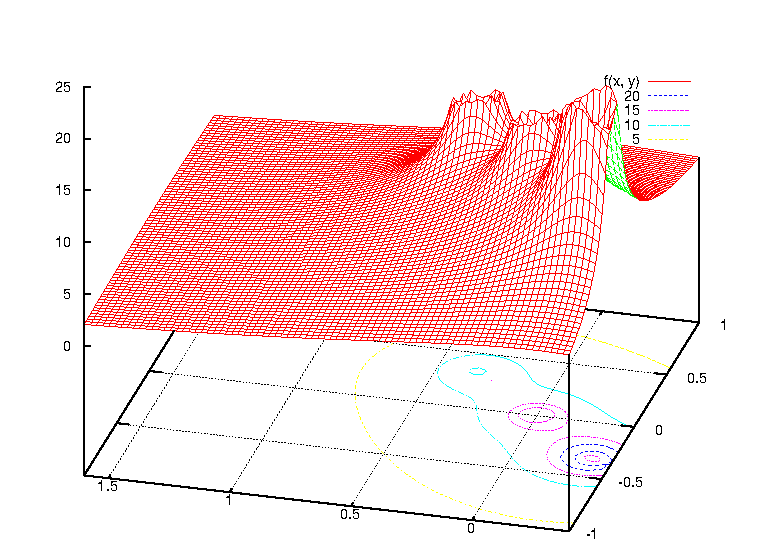
\includegraphics[width=.75\textwidth]{fig/exemplo1.eps}
\caption{\label{fig:fig2}This is another figure}
\end{figure}

Duis autem vel eum iriure dolor in hendrerit in vulputate velit
esse molestie consequat vel illum dolore eu feugiat nulla
facilisis at vero eros et accumsan et iusto odio dignissim qui
blandit praesent luptatum zzril delenit augue duis dolore te
feugait nulla facilisi lorem ipsum dolor sit amet consectetuer
adipiscing elit sed diam nonummy nibh euismod tincidunt ut laoreet
dolore magna aliquam erat volutpat.

Ut wisi enim ad minim veniam quis nostrud exerci tation
ullamcorper suscipit lobortis nisl ut aliquip ex ea commodo
consequat duis autem vel eum iriure dolor in hendrerit in
vulputate velit esse molestie consequat vel illum dolore eu
feugiat nulla facilisis at vero eros et accumsan et iusto odio
dignissim qui blandit praesent luptatum zzril delenit augue duis
dolore te feugait nulla facilisi.

Nam liber tempor cum soluta nobis eleifend option congue nihil
imperdiet doming id quod mazim placerat facer possim assum lorem
ipsum dolor sit amet consectetuer adipiscing elit sed diam nonummy
nibh euismod tincidunt ut laoreet dolore magna aliquam erat
volutpat ut wisi enim ad minim veniam quis nostrud exerci tation
ullamcorper suscipit lobortis nisl ut aliquip ex ea commodo
consequat.

\subsection{Another subsection}

lorem ipsum dolor sit amet consetetur sadipscing elitr sed diam
nonumy eirmod tempor invidunt ut labore et dolore magna aliquyam
erat sed diam.~\cite{COFFMANPACKING98}

\subsubsection{Another subsubsection}

lorem ipsum dolor sit amet consetetur sadipscing elitr sed diam
nonumy. A seguir, a Tabela~\ref{tab:tab2} mostra algo mais
simples.

% Um exemplo de tabela mais simples.
\begin{table}
\begin{center}%
\caption{\label{tab:tab2}Note que a legenda da tabela fica na parte de cima}%
%\setlength{\tabcolsep}{1cm}%
\begin{tabular*}{.7\linewidth}{@{\extracolsep{\fill}}lll}%
\noalign{\smallskip}
\hline
lorem & ipsum & dolor \tabularnewline
sit & amet & consetetur \tabularnewline
sadipscing & elitr & sed \tabularnewline
diam & nonumy & eirmod \tabularnewline
tempor & invidunt & ut \tabularnewline
labore & et & dolore \tabularnewline
magna & aliquyam & erat \tabularnewline
sed & diam & voluptua \tabularnewline
at & vero & eos \tabularnewline
\end{tabular*}
\end{center}
\end{table}

Lorem ipsum dolor sit amet consetetur sadipscing elitr sed diam
nonumy eirmod tempor invidunt ut labore et dolore magna aliquyam
erat sed diam voluptua at vero eos et accusam et justo duo dolores
et ea rebum stet clita kasd gubergren no sea takimata sanctus est
lorem ipsum dolor sit amet lorem ipsum dolor sit amet consetetur
sadipscing elitr sed diam nonumy eirmod tempor invidunt ut labore
et dolore magna aliquyam erat sed diam voluptua at.

Lorem ipsum dolor sit amet consetetur sadipscing elitr sed diam
nonumy eirmod tempor invidunt ut labore et dolore magna aliquyam
erat sed diam voluptua at vero eos et accusam et justo duo dolores
et ea rebum stet clita kasd gubergren no sea takimata sanctus est
lorem ipsum dolor sit amet lorem ipsum dolor sit amet consetetur
sadipscing elitr sed diam nonumy eirmod tempor invidunt ut labore
et dolore magna aliquyam erat sed diam voluptua at.


%----------------------------------------------------------------
% Aqui vai a bibliografia. Existem 3 estilos de citação: use
% 'tcc-alpha' para citações do tipo [Abc+] ou [XYZ] (em ordem
% alfabética na bibliografia), 'tcc-num' para citações
% numéricas do tipo [1], [20], etc., em ordem de referência e
% 'tcc-alpha-full' para citações estilo 'alpha' mas com nomes completos.
%----------------------------------------------------------------
\bibliographystyle{tcc-alpha}
%\bibliographystyle{tcc-num}
\bibliography{exemplo-bib}

%----------------------------------------------------------------
% Após \appendix, se iniciam os capítulos de Apêndice, com
% numeração alfabética.
%----------------------------------------------------------------
\appendix
\chapter{Meu primeiro apêndice}
\chapter{My second appendix}

%----------------------------------------------------------------
% Aqui vão os "capítulos" de anexos. Cada anexo deve
% ser considerado um capítulo.
%----------------------------------------------------------------
\anexos
\chapter{Meu primeiro anexo}
\chapter{My second attachment}

% E aqui (para a felicidade de todos) termina o documento.
\end{document}
